\documentclass[cs4size,a4paper]{ctexart}   
\usepackage{amlnote}
\usepackage{dirtree}
\usepackage{tikz}
\usetikzlibrary{shapes.geometric, arrows}
%===正文开始===
\begin{document}

\fancyhead[C]{\zihao{5} \kaishu 编译原理项目作业报告}
%===首页===
\begin{titlepage}
\begin{center}
% Upper part of the page
\includegraphics[width=0.30\textwidth]{logo}\\[1cm]    
\textsf{\LARGE\bfseries 编译原理项目报告}\\[1.0cm]
\textsc{\Large 2022-2023学年第2学期}\\[0.5cm]
% Title
\HRule \\[0.8cm]
{\huge \bfseries 基于 C 语言的编译器简易实现}\\[0.4cm]
\HRule \\[0.7cm] 
% Author
\textsc{计科2003-2020040227-谭植文(组长)}\\[0.4cm]
\textsc{计科2004-2020040177-刘晔宁}


\vfill
% Bottom of the page
{更新日期:\today}
\newpage
\tableofcontents 
\end{center}
\end{titlepage}


%===第一章===
\section{前言}
{\par 在编译原理课程的学习中,了解到编译器主要的工作原理,我们小组根据在此学习的基础上,完成课程项目作业。}
\section{项目目标}
{\par 本项目的目标是实现一个简单的 C 语言编译器。}
\begin{itemize}
    \item 词法分析
    \item 语法分析
    \item 语义分析
    \item 中间代码生成
    \item 代码优化
    \item 目标代码生成
\end{itemize}
\section{开发环境}
\begin{itemize}
    \item 操作系统:Windows 11
    \item 开发工具:Visual Studio Code
    \item 开发语言:C++
    \item 编译器:MinGW 8.1.0
    \item graphviz 8.0.3
\end{itemize}
\section{实现方法}(基本思路、解决的问题和手段、关键算法和处理流程等)
\subsection{主程序}
\subsubsection{基本思路}
\begin{enumerate}
    \item 读取词法文件,生成对应的 DFA
    \item 读取源文件,对源文件进行词法分析,输出 token 序列
    \item 根据语法文件,生成 LR(1) 分析表
    \item 根据 token 序列作为输入,进行语法分析,输出语法生成树
    \item 遍历语法树,递归进行语义分析,输出语义分析结果
\end{enumerate}
\subsubsection{算法流程}
\begin{lstlisting}[language=c++]
// 词法分析
while 读取词法文件:
    生成对应的 DFA 
while 读取源文件:
    if 当前字符为字母:
        识别标识符
    else if 当前字符为数字:
        识别数字
    else if 当前字符为运算符:
        识别运算符
    else if 当前字符为界符:
        识别界符
    else:
        识别错误
输出词法分析结果 token 序列

//语法分析
while 读取语法文件:
    生成 LR(1) 分析表
将 token 序列作为输入,进行语法分析
输出语法分析结果

//语义分析
遍历语法树,递归进行语义分析

\end{lstlisting}
\subsubsection{解决问题}
\begin{itemize}
    \item 识别界符时,需要考虑界符的组合,如\lstinline{<=}、\lstinline{>=}、\lstinline{==}、\lstinline{!=}、\lstinline{&&}、\lstinline{||}等
    \item 对于某些界符,需考虑与 DFA 生成时所需的符号是否产生冲突,例如\lstinline{`}、\lstinline{*}、\lstinline{(}、\lstinline{)}、\lstinline{|}等。利用其他符号做替换
\end{itemize}
\subsection{词法分析}
\subsubsection{基本思路}
\begin{enumerate}
    \item 将正则表达式转换为后缀表达式
    \item 将后缀表达式转换为 NFA
    \item 将 NFA 转换为 DFA
    \item 最小化 DFA
    \end{enumerate}
\subsubsection{算法流程}
\begin{lstlisting}[language=c++]
// 正则表达式转为后缀表达式
建立运算符栈用于运算符的存储,此运算符遵循越往栈顶优先级越高的原则
while 扫描表达式:
    if 当前字符是字母(优先级为0的符号):
        直接输出
    else if 当前字符为运算符或者括号(优先级不为0的符号),则判断:
        if 当前运算符为'(':
            直接入栈
        else if ')':
            出栈并顺序输出运算符直到遇到第一个'(',遇到的第一个'('出栈但不输出;
        else:
            if 栈顶元素是'(':
                当前元素直接入栈;
            else if 栈顶元素优先级 >= 当前元素优先级:
                while(栈顶元素优先级>当前元素优先级):
                    出栈并顺序输出运算符
                当前元素入栈
            else if 栈顶元素优先级<当前元素优先级:
                当前元素直接入栈
顺序出栈并输出运算符直到栈元素为空

// 后缀表达式转为 NFA
建立状态栈用于存储状态,建立状态转换表用于存储状态转换关系
while 读取后缀表达式:
    if 元素是字符:
        创建两个状态,分别作为状态转换表的起始状态和终止状态
        将状态对入栈
    else if 元素是'|':
        创建两个状态,分别作为状态转换表的起始状态和终止状态
        从栈中取两个状态对
        根据法则进行链接
        将状态对入栈
    else if 元素是'*':
        创建两个状态,分别作为状态转换表的起始状态和终止状态
        从栈中取两个状态对
        根据法则进行链接
        将状态对入栈
    else if 元素是'`':
        创建两个状态,分别作为状态转换表的起始状态和终止状态
        从栈中取状态对
        根据法则进行链接
        将状态对入栈

// NFA 转 DFA
建立 DFA 状态集合,用于存储 DFA 的状态
建立 DFA 状态队列
NFA 开始状态闭包入队
while 队列非空:
    取队首状态闭包
    for 每个输入符号:
        计算输入符号对应的状态闭包
        if 该状态闭包不在 DFA 状态集合中:
            将该状态闭包加入 DFA 状态集合
            将该状态闭包入队
        记录状态闭包对应的 DFA 状态
        记录状态闭包对应的 DFA 状态转换
    出队

// 最小化 DFA
建立最小化分析表
将非终态和终态分别编号为 0 和 1
while 新生成状态不同:
    根据 DFA 状态转换表将状态分为不同的等价类
    根据等价类,生成新的 DFA 状态转换表
    根据新的 DFA 状态转换表生成新的 DFA 状态集合
\end{lstlisting}
\subsubsection{解决问题}
\begin{itemize}
    \item 对于图的数据结构的设计,最开始将状态和边分别存储,这样会导致遍历时需要多次循环,效率低下。最终更改为邻接表的存储,提高了效率。
    \item 在寻找闭包等需要递归操作时,采用了队列的方式,将递归转换为迭代,提高了效率。
    \item 最小化 DFA 时,路径的对应关系复杂,容易出错
\end{itemize}
\subsection{语法分析}
\subsubsection{基本思路}
\begin{enumerate}
    \item 采用 LR(1) 分析法
    \item 对文法进行拓广
    \item 根据文法构建 DFA 
    \item 根据 DFA 构建 LR(1) 分析表
\end{enumerate}
\subsubsection{算法流程}
\begin{lstlisting}[language=c++]
// 对文法进行拓广
增加一个新的开始符号 S' 和一个新的产生式 S' -> S

// 根据文法构建 DFA
建立状态栈用于存储状态,建立状态转换表用于存储状态转换关系
构建开始状态闭包以及对应搜索符
while 有新状态生成:
    for 每一条产生式:
        根据 dot 位置和搜索符计算新状态闭包
        if 状态核心项相同:
            指向该状态
        else:
            新建状态

// 根据 DFA 构建 LR(1) 分析表
建立 LR(1) 分析表
\end{lstlisting}
\subsubsection{解决问题}
\begin{itemize}
    \item 在寻找相同状态时,应当是核心项中所有产生式完全相同,之前产生错误即只比较了其中一项,导致状态减少
    \item 在求解 First 和 Follow 集合时,需要考虑空串的情况,即将当前符号后所有符号遍历
    \item 在构建 DFA 时,状态添加新文法需要将文法闭包添加到状态闭包中,否则会出现错误
\end{itemize}
\subsection{语义分析}
\subsubsection{基本思路}
\begin{enumerate}
    \item 采用递归下降分析法
    \item 遍历语法树,递归进行语义分析
    \item 采用深度优先遍历
\end{enumerate}
\subsubsection{算法流程}
\begin{lstlisting}[language=c++]
void DFA(root):
    if root is leaf:
        root.value = token.value
    for each child:
        DFA(child)
        root.value = root.value + child.value
\end{lstlisting} 
\section{结果}(界面和使用方法、实际例子的输入输出效果)
\subsection{文件目录结构}
\dirtree{%
.1 compiler.
.2 grammer\_analysis.
.3 include.
.3 src.
.2 input.
.3 grammer.txt.
.3 lextion.txt.
.2 lexical\_nalysis.
.3 include.
.3 src.
.2 output.
.3 analysis\_process.txt.
.3 grammer\_tree.dot.
.3 lex\_result.txt.
.2 report.
.2 main.cpp.
.2 sample.tan.
.2 .gitignore.
.2 CmakeLists.txt.
}



\subsection{使用方法}
\begin{enumerate}
    \item 在终端打开根目录
    \item 依次输入以下命令
            \begin{lstlisting}
mkdir build
cmake -G "MinGW Makefiles" -Bbuild . //-G参数指定生成器,可以去掉
cd build
make
            \end{lstlisting}
    \item 在根目录下会生成 main.exe
    \item 终端回到根目录,运行程序
        \begin{lstlisting}
cd ..
./main.exe
        \end{lstlisting}
\end{enumerate}
\subsection{实际例子的输入输出效果}
\subsubsection{输入}
\begin{itemize}
    \item 词法分析 ./input/lexicon.txt
    \item 语法分析 ./input/grammer.txt
    \item 分析源程序 ./sample.tan
    \begin{lstlisting}
int main(int argc, char* argv[100])  
{  
    static double pi = 3;
    const int a = 7;
    const int b = 9;
    int c = a+b;
    int d[10] = {6,54,52,34,55,68,10,90,78,56};
    int i;
    int sum=0;

    if(a+b>10)
    {
        printf("true");
    }
    else
    {
        printf("false");
    }

    for (i=0;i<10;i++)  
    {  
        sum=sum+d[i];
    }

    printf(c);
    printf(sum);  
    printf("HelloWorld");  
    return 0;  
}  
    \end{lstlisting}
\end{itemize}
\subsubsection{输出}
\begin{itemize}
    \item token 序列 ./output/lex\_result.txt
    \item 分析过程 ./output/analysis\_process.txt
    \item 语法树 ./output/grammer\_tree.txt
    \begin{figure}[htpb] 
        \centering
        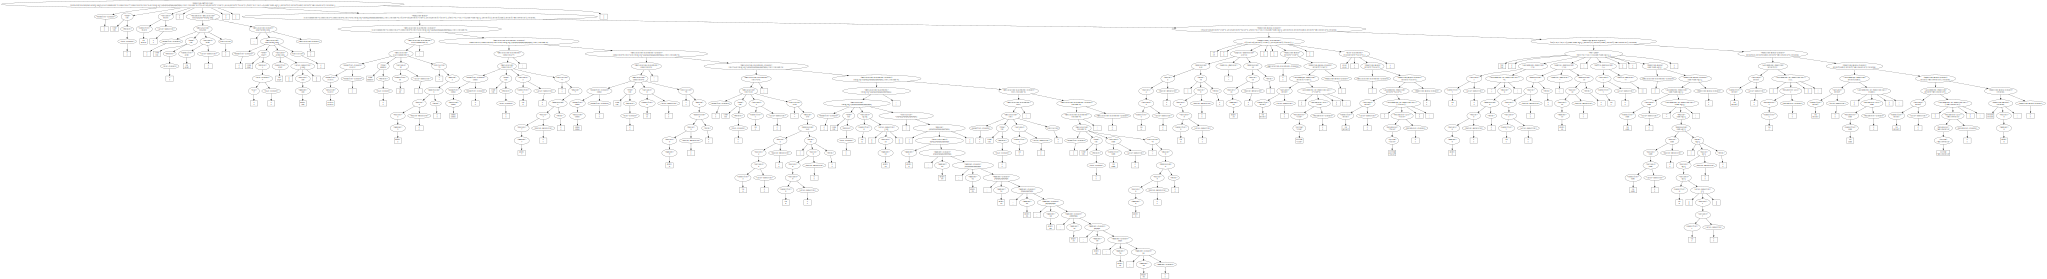
\includegraphics[width=0.8\linewidth]{./figure/grammer_tree.png}
        \caption{语法树缩略图}
    \end{figure}
\end{itemize}
\subsubsection{查看语法树}
\begin{enumerate}
    \item 安装 Graphviz
    \item 在终端打开output目录
    \item 在终端输入以下命令
            \begin{lstlisting}
// 图片较大,建议生成 svg 图片,也可根据需要生成对应的格式
// 复制命令注意符号格式不同
dot -Tsvg grammer_tree.dot -o grammer_tree.svg 
                \end{lstlisting}
\end{enumerate}
\section{项目分工}
\begin{itemize}
    \item 谭植文\ 65\%:\\
        主要完成了主程序、词法分析和语法分析的代码编写
    \item 刘晔宁\ 35\%:\\
        主要完成了词法分析规则、部分 C 语言文法和报告的攥写
\end{itemize}
%===参考文献===
%\addcontentsline{toc}{section}{参考文献}
%\bibliographystyle{abbrv}     %论文引用格式
%\bibliography{E:/studio/wrtex/wrtkit/referbib/citavi}
                         
\begin{thebibliography}{99}
\bibitem{A23a}
Author. Article Title. \url{http://www.arxiv.org}, 2023.

\bibitem{B23b}
Author. Project. \url{http://www.baidu.com}, 2023.

\bibitem{B23b}
Author. 网络笔记标题. \url{https://blog.csdn.net}, 2023.
\end{thebibliography}
\end{document}
%===结束===




